% Marco Teórico
\chapter{Marco teórico}

En este capítulo se presentan los conceptos y recursos utilizados en el proyecto. En las \textbf{secciones \ref{sec:ld}} y \textbf{\ref{sec:contrdi}}, se habla sobre la teoría de lógica difusa y controladores difusos respectivamente; \textbf{La sección \ref{sec:sde}} trata el concepto de sistemas difusos evolutivos; la \textbf{sección \ref{sec:orbex}} presenta la librería de lógica difusa que se utilizó para desarrollar el sistema de aprendizaje; la pista y el vehículo utilizado para las pruebas se introducen en las \textbf{secciones \ref{sec:zoco}} y \textbf{\ref{sec:carros}}; por último la sección \textbf{\ref{sec:carros}} trata sobre el simulador utilizado durante la realización del proyecto.   

\section{Lógica difusa} 
\label{sec:ld}
En la década de los 60, Lotfi Zadeh, un profesor matemático iraní residente en los Estados Unidos, describe los fundamentos matemáticos asociados a la teoría de conjuntos difusos y por extensión a la lógica difusa (\textit{Fuzzy logic}) \cite{zadeh1965fuzzy}.

La lógica difusa es una lógica multievaluada, que en vez de trabajar con el modelo clásico de inclusión y exclusión, remplaza los dos valores de veracidad verdadero y falso ($\{0,1\}$), por un continuo de valores, generalmente representados por el intervalo $[0,1]$. 

Una de las principales aplicaciones de la lógica difusa es el modelado del razonamiento humano en situaciones donde se posee información vaga, incompleta y/o (parcialmente) contradictoria; normalmente en la forma de sistemas basados en reglas. 

Los conjuntos difusos, que están basados en esta lógica, pueden ser utilizados para modelar la vaguedad lingüística escondida en atributos como \textit{grande} y \textit{pequeño} y, en particular, la transición gradual entre ellos. Éstos se presentan a continuación.


\subsection{Conjuntos difusos}
\label{sec:cd}

La teoría de conjuntos difusos expresa imprecisiones de manera cuantitativa, por medio de introducir una función que refleja el grado de pertenencia de un valor hacia un atributo, adoptando valores que pertenecen al intervalo [0,1].

Un conjunto difuso es un par $(A,m)$ donde $A$ es un conjunto y $m : A \longrightarrow [0,1]$.
Para cada $x \in A, m(x)$ es llamado el grado de pertenencia de $x$ en $(A,m)$.

\begin{figure}[htb]
\centering
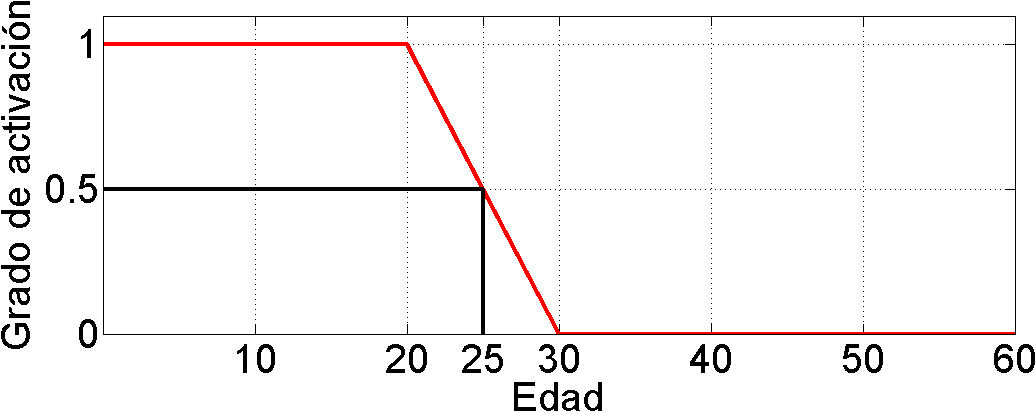
\includegraphics[width=0.55\textwidth,type=png,ext=.png,read=.png]{figures/conjunto_difuso}
\caption{Conjunto difuso que representa a grupo de personas jóvenes.}
\label{fig:conjunto}
\end{figure} 

En la figura \ref{fig:conjunto} se observa un ejemplo del conjunto difuso que representaría a las personas \textit{jóvenes}. De 0 a 20 años diríamos que las personas pertenecen completamente al grupo de gente joven, pero a medida que va aumentando la edad, va reduciendo su grado de pertenencia al conjunto de los jóvenes. De esta forma, con unos 25 años todavía se seria joven al 50 \%, y a partir de 30 años dejaría de pertenecer al grupo. 

En los sistemas de control basados en lógica difusa, la forma más común utilizada en las funciones de pertenencia es el triángulo, aunque otras como los trapecios y la curva de bell también son muy utilizados. De tres a siete curvas es generalmente apropiado para cubrir los rangos sobre los  que se están trabajando, así como no supone un esfuerzo notable para el diseñador, el trabajar con ellas. 

\begin{figure}[htb]
\centering
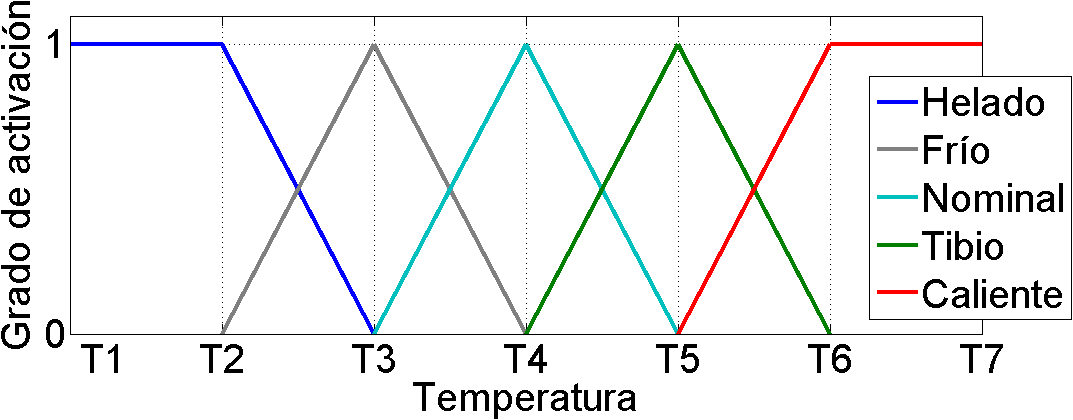
\includegraphics[width=0.55\textwidth,type=png,ext=.png,read=.png]{figures/fpertenencia}
\caption{Sistema difuso correspondiente a la temperatura, con cinco funciones de pertenencia. Cada etiqueta o función de pertenencia corresponde a un nivel de temperatura.}
\label{fig:fpertenencia}
\end{figure} 

%Puedes quitar esto(es opcional)

\section{Controladores difusos} 
\label{sec:contrdi}


Los controladores difusos aplican la teoría de conjuntos difusos para definir y resolver problemas de control. Contienen una colección de funciones de pertenencia y reglas que son utilizadas para razonar sobre datos. Trabajan de una manera diferente a los controladores convencionales, ya que utilizan el conocimiento experto en lugar de ecuaciones diferenciales para describir un sistema y su comportamiento. 

Dicho conocimiento se representa de manera natural,  por medio del uso de variables lingüísticas que representan conjuntos difusos; describiendo así, el conocimiento de una manera similar a como lo haría un experto. 

Se define la \textbf{topología del controlador} como la cantidad, forma que poseen y la manera en que se encuentran distribuidas, las etiquetas o funciones de pertenencias, que han sido asignadas a lo largo de los rangos establecidos para cada una de las variable de entrada.

Su funcionamiento se descompone en una etapa de entrada, una de procesamiento y una de salida. En la \textbf{etapa de entrada}, se asignan los grados de pertenencia a los conjuntos difusos correspondientes, en función de los valores de entrada. La \textbf{etapa de procesamiento} evalúa las reglas involucradas y genera un grado de veracidad a las mismas, para luego combinar el resultado de las reglas. Finalmente, la \textbf{etapa de salida} convierte el resultado obtenido en un valor salida específico. 

Los sistemas difusos están formados principalmente por cuatro componentes, y siguen un esquema como el que se presenta en la figura \ref{fig:controlador}. 
Cada una de las etapas que definen el funcionamiento de un controlador difuso se detallan en las siguientes subsecciones.


\begin{figure}[htb]
\centering
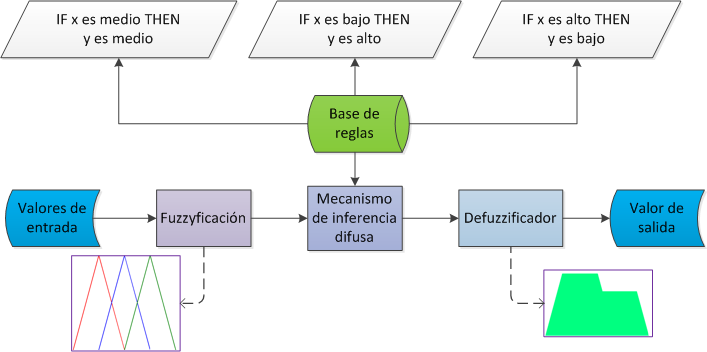
\includegraphics[width=0.7\textwidth,type=png,ext=.png,read=.png]{figures/sistemad}
\caption{Esquema de procesamiento general de un sistema difuso.}
\label{fig:controlador}
\end{figure} 



\subsection{Fuzzificador}


La entrada de un sistema basado en lógica difusa es, por lo general, un valor numérico. Para que este valor pueda ser procesado por el sistema difuso se hace necesario convertirlo a un \textit{lenguaje}  para que el mecanismo de inferencia pueda procesarlo. 

La función del \textit{fuzzificador} es la de realizar tal conversión. Éste toma los valores numéricos provenientes del exterior y los convierte en valores \textit{difusos} para que puedan ser procesados por el mecanismo de inferencia. Estos valores difusos están representados por los grados de pertenencia de los valores de entrada a los diferentes conjuntos difusos en los que se ha dividido el universo de discurso de cada una de las variables de entrada.


\subsection{Mecanismo de inferencia difusa}


Teniendo los diferentes niveles de pertenencia arrojados por el fuzzificador, los mismos deben ser procesados para general una salida difusa. La tarea del sistema de inferencia es tomar los niveles de pertenencia y apoyado en la base de reglas generar la salida del sistema difuso.


\subsection{Reglas de control difuso}


La base de reglas es la manera que tiene el sistema difuso de almacenar el conocimiento lingüístico que le permite resolver el problema para el cual ha sido diseñado.

Describe la metodología o el conjunto de reglas que aplicaría un ser humano encargado de controlar el proceso, con toda la imprecisión que poseen los lenguajes naturales y, sólo a partir de estas reglas, generar las acciones de control. La base de reglas se representa mediante un conjunto de reglas del tipo:

\begin{center}
\begin{alltt}
IF \textit{x1} es pequeño AND \textit{x2} es grande THEN \textit{y} es medio 
IF \textit{x1} es pequeño AND \textit{x2} es medio THEN \textit{y} es grande 
\end{alltt}
\end{center} 

Estas expresiones de la forma \textit{IF...THEN...} son las reglas de control difuso. Las variables de condición $x1, x2, ...,$ representan las variables de entrada del sistema, y se ubican en el antecedente; la variable $y$ es la salida del mismo, y pertenece al consecuente, las palabras \textit{pequeño}, \textit{grande} y \textit{medio} son los conjuntos difusos en los que se codifica la variable de entrada.

Los controladores difusos contienen grupos de reglas y actúan de la forma siguiente: Cuando se les proporciona el valor actual de las variables de entrada se obtiene el valor de verdad de las reglas, calculado mediante un método de \textit{inferencia difusa}. 

Teniendo en cuenta que los sistemas de control deben actuar en tiempo real, los métodos de inferencia que se usan suelen ser sencillos y rápidos.  


\subsection{Defuzzificador}


La salida que genera el mecanismo de inferencia es una salida difusa, por lo que no puede ser interpretada por un elemento externo (por ejemplo un controlador) que solo manipule información numérica. 

Para lograr que la salida del sistema difuso pueda ser interpretada por elementos que sólo procesen información numérica, hay que convertir la salida difusa en un valor numérico; este proceso lo realiza el \textit{defuzzificador}. Para generar la salida numérica a partir de este conjunto existen varias opciones como el Centro de Gravedad, los Centros Promediados entre otros.

\section{Sistemas difusos evolutivos} 
\label{sec:sde}

Pueden definirse como sistemas de auto-desarrollo y auto-aprendizaje basados en lógica difusa, en los cuales, tanto sus parámetros como su estructura, alcanzan un estado de auto-adaptación \textit{on-line}.

Generalmente son asociados con flujo de datos y modos de operación \textit{on-line} (a menudo en tiempo real). Pueden ser vistos como sistemas difusos adaptativos. La diferencia es que los sistemas difusos evolutivos asumen la adaptación en línea de la estructura del sistema, ademas de la adaptación de parámetros, que es usualmente asociada con el termino adaptativo. También permiten la adaptación del mecanismo de aprendizaje. De esta manera, evolutivo asume un nivel superior a adaptativo. 

Uno de los problemas de los controladores (particularmente los controladores difusos), es el diseño y la configuración precisa. Debido al cambio constante en el ambiente de operación de las plantas industriales y los controladores, el diseño y configuración \textit{off-line} no proporciona la flexibilidad que es requerida. La teoría de control adaptativo nos provee con una manera para resolver esta situación, basada en la adaptación constante de los parámetros del (usualmente linear) controlador. Los problemas reales, generalmente no son lineales, ni estacionario, por lo tanto, la teoría de control adaptativa, tiene sus obvias limitaciones.
 
Los controladores difusos evolutivos basados en reglas \cite{angelov04}\cite{Angelov02}, combinan la flexibilidad y naturaleza no linear de los sistemas difusos, con las ventajas de los esquemas adaptativos bien establecidos.  

\section{ORBEX} 
\label{sec:orbex}

Los controladores utilizados por el programa de control utilizado en el grupo AUTOPIA están definidos utilizando la librería de modelado difuso \gls{ORBEX} \cite{Garcia1998}, la cual sigue un esquema como el que se presenta en la sección \ref{sec:contrdi}. El entorno ha sido usado por el grupo AUTOPIA para el modelado y ejecución en tiempo real de los controladores difusos que controlan los vehículos. 

Con los controladores definidos por \gls{ORBEX}, se pueden describir diferentes formas de conducción con el fin de emular comportamientos de diferentes tipos de conductores y adaptar la conducción a la situación actual del tráfico. Dichas estrategias pueden ser definidas e implementadas mediante reglas difusas del tipo \textit{IF...THEN...}

\gls{ORBEX} trabaja con controladores difusos que utilizan funciones de pertenencia trapezoidales para la codificación de las variables de entrada, y \textit{\gls{singletons}} para la codificación de variables de salida. Esto permite tomar decisiones de control en un período de tiempo muy corto, con muy buena precisión y garantizando la estabilidad del sistema. 

Los \textbf{singletons} son conjuntos que poseen un único elemento, se utilizan como el consecuente de las reglas difusas que definen al controlador. Representan el valor que va ha ser aplicado, una vez que se active, o se cumpla, la regla correspondiente.

Para el diseño de un controlador con \gls{ORBEX} es necesario especificar 3 secciones fundamentales:
\begin{itemize}
    
    \item Las variables de entrada al sistema con sus respectivas particiones difusas o etiquetas lingüísticas.
    
    \item Las variables de salida del sistema con sus respectivas particiones (\gls{singletons}). 
    
    \item Un conjunto de reglas de inferencia que operan sobre las variables de entrada y de salida de tal forma que a las variables de salida les sea asignado un valor.
\end{itemize}

El número de reglas de los controladores que se utilizaron en el proyecto, es igual al producto entre el número de etiquetas o funciones de pertenencia que hallan sido asignadas a cada variable de entrada, por lo la base de datos de las reglas presenta un crecimiento exponencial al insertarse una nueva etiqueta. Una regla de un controlador con dos variables de entradas es de la siguiente forma:

\begin{center}
{\tt SI Entrada0 ET01 Y Entrada1 ET12 ENTONCES Pedal Ped5} \hspace{4 cm}(2.1)
\end{center} 

Donde \verb,Entrada0, y \verb,Entrada1, son los valores de entrada. \verb,ET01, es la etiqueta o función de pertenencia número uno de la variable de entrada cero, y \verb,ET12, es la etiqueta dos de la variable de entrada uno, ambas etiquetas poseen forma trapezoidal, se definen especificando el valor de las coordenada en el eje $x$ de cada vértice del trapecio, las coordenada en $y$ son asignadas automáticamente por \gls{ORBEX}, siendo cero para el primer y último valor, y  uno para el segundo y el tercero. \verb,Ped5, es el singleton que representa el consecuente de la regla, es el valor que se debe aplicar cuando e activa o se cumple con un cierto grado esta regla, un posible valor para \verb,Ped5, puede ser -0.10552.  

Para una explicación más detallada sobre el diseño de controladores con \gls{ORBEX}, referirse a la sección \ref{ape:diseno} del apéndice.

La gramática de \gls{ORBEX} (ver apéndice \ref{ape:gramatica}), nos permite el uso de modificadores lingüísticos, éstos se presentan en la tabla \ref{modificadores}, cada uno con su función de cómputo asociada, donde $\mu$ representa el grado de pertenencia del valor de la variable de entrada a un determinado subconjunto difuso.

\begin{table}[htb]
  \centering
  \begin{tabular}{|c|c|}
    \hline
    % after \\: \hline or \cline{col1-col2} \cline{col3-col4} ...
    \rowcolor[gray]{0.9} \textbf{Modificador} & \textbf{Cálculo} \\
    \hline
    \hline
    \textit{POCO} & $\sqrt{\mu}$ \\ \hline
    \textit{MUY} & $\mu^{2}$ \\ \hline
    \textit{EXTRA} & $\mu^{3}$ \\ \hline
    \textit{MAYORQUE(a)} & $\mu_{>a}$ = 1 - $\mu_{a}$\\ \hline
    \textit{MENORQUE(a)} & $\mu_{<a}$ = 1 - $\mu_{a}$ \\ \hline
    \textit{ENTRE(a,b)} & MAYORQUE(a) x MENORQUE(b) \\ \hline
    \textit{NO} & 1-$\mu$ \\
    \hline
  \end{tabular}
  \caption{Modificadores Lingüísticos soportados por ORBEX}
  \label{modificadores}
\end{table}

En la sección \ref{ape:orbex} del apéndice se presenta un ejemplo de un controlador definido en \gls{ORBEX}.

Otro aspecto a tener en cuenta sobre el proceso de inferencia usado por \gls{ORBEX}. Una vez establecido el valor de las variables de entrada, el sistema realiza el proceso de \textit{fuzzificación}, que asigna un valor de pertenencia a cada subconjunto o partición difusa de la variable según el valor \textit{crisp} asignado a la variable. Una vez hecho esto, se procede a la inferencia, que sigue el siguiente procedimiento estándar para cada una de las reglas:

\begin{enumerate}
    \item Se calcula primero el grado de cumplimiento de la primera condición
    \item Se asigna este cumplimiento a una variable temporal \{\textit{W}\}
    \item Se calcula el grado de cumplimiento de la segunda condición
    \item Se calcula el conectivo lógico \{\textit{Y/O}\} mediante las t-normas y s-normas mínimo y máximo
    \item Se guarda el resultado en la variable temporal \{\textit{W}\}
    \item Se calcula el grado de cumplimiento de la tercera condición
    \item Se calcula el conectivo lógico \{\textit{Y/O}\} mediante las t-normas y s-normas mínimo y máximo
    \item Así, en general para \textit{N} condiciones y conectivos lógicos.
\end{enumerate}

El valor final de la variable temporal \{\textit{W}\} representará el grado de satisfacción del antecedente de la regla y que este valor será el peso que se asigne al consecuente de la regla. Una vez realizado el proceso de inferencia, se pasa al proceso de \textit{defuzzificación}, que consiste en la suma ponderada de los singletons de la variable de salida, según la siguiente fórmula $\frac{\sum P_{i}w_{i}}{\sum w_{i}}$,
donde $w_{i}$ es el peso correspondiente a la partición difusa singleton $P_{i}$.

%\begin{equation}
%    \frac{\sum P_{i}w_{i}}{\sum w_{i}}
%\end{equation}
%\noindent donde $w_{i}$ es el peso correspondiente a la partición difusa singleton $P_{i}$.

\section{ZOCO}
\label{sec:zoco}

\gls{ZOCO} es una pista de pruebas de vehículos automáticos que está dedicada exclusivamente a tareas de
investigación, es decir, en ella no hay ningún otro tráfico de vehículos, lo que se ha hecho por razones de seguridad. Tiene una
forma reticulada, como las manzanas o cuadras de una ciudad, con algunas irregularidades, con calles de seis metros de ancho,
permite la circulación en ambos sentidos. En la figura \ref{fig:zoco} se puede ver una vista aérea de \gls{ZOCO}\footnote{Fuente: \url{http://maps.google.es}}.

Las calles horizontales tienen nombres de personajes dedicados a la automatización, mientras que las verticales están dedicadas a antiguos científicos y personajes que diseñaron y crearon instrumentos de navegación (ver anexo \ref{ape:zoco}).

\begin{figure}[h]
  \centering
  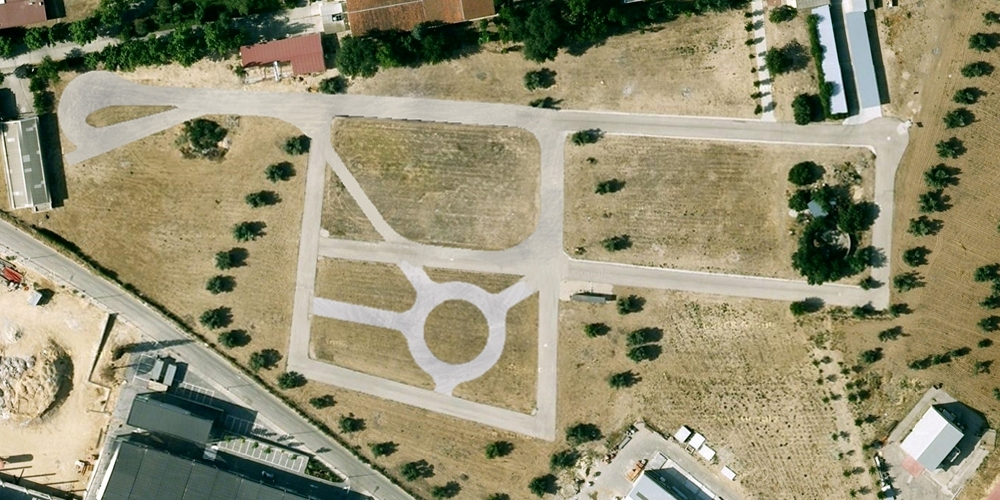
\includegraphics[width=0.5\textwidth]{figures/zoco.png}
  \label{zoco}
  \caption{Vista aérea de ZOCO}
  \label{fig:zoco}
\end{figure}

Estos nombres de calles nos permiten especificar los recorridos que han de hacer los coches de una manera simbólica, estos recorridos son transformados por un intérprete en un conjunto de maniobras elementales, evidentemente, el intérprete ha de poseer un mapa de \gls{ZOCO}.

\gls{ZOCO} también dispone de una estación base de posicionamiento global diferencial basado en información geográfica vía satélite, \gls{DGPS}, que puede ser utilizado por sistemas móviles embarcados en los coches para obtener su posición con una precisión inferior al centímetro \cite{Milanes2008a} \cite{Milanes2008b}. 

Existe una estación central de coordinación sobre la que se prueban las estrategias, normalmente basadas en lógica difusa, que luego son transferidas a los coches \cite{GodoyBilbao2010}.

\section{Vehículos automatizados}
\label{sec:carros}

La flota de vehículos del grupo AUTOPIA esta formada por 5 automóviles (ver sección \ref{ape:carros} en el anexo), de los cuales utilizaremos un \textbf{Citroën C3 Pluriel}, llamado \textbf{Platero}, para realizar las pruebas experimentales del sistema desarrollado en este trabajo.

\begin{figure}[ht]
\begin{minipage}[b]{0.5\linewidth}
\centering
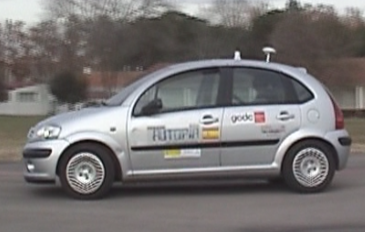
\includegraphics[width=0.9\linewidth]{figures/platero.png}
\caption{Platero}
\label{fig:platero}
\end{minipage}
\begin{minipage}[b]{0.5\linewidth}
\centering
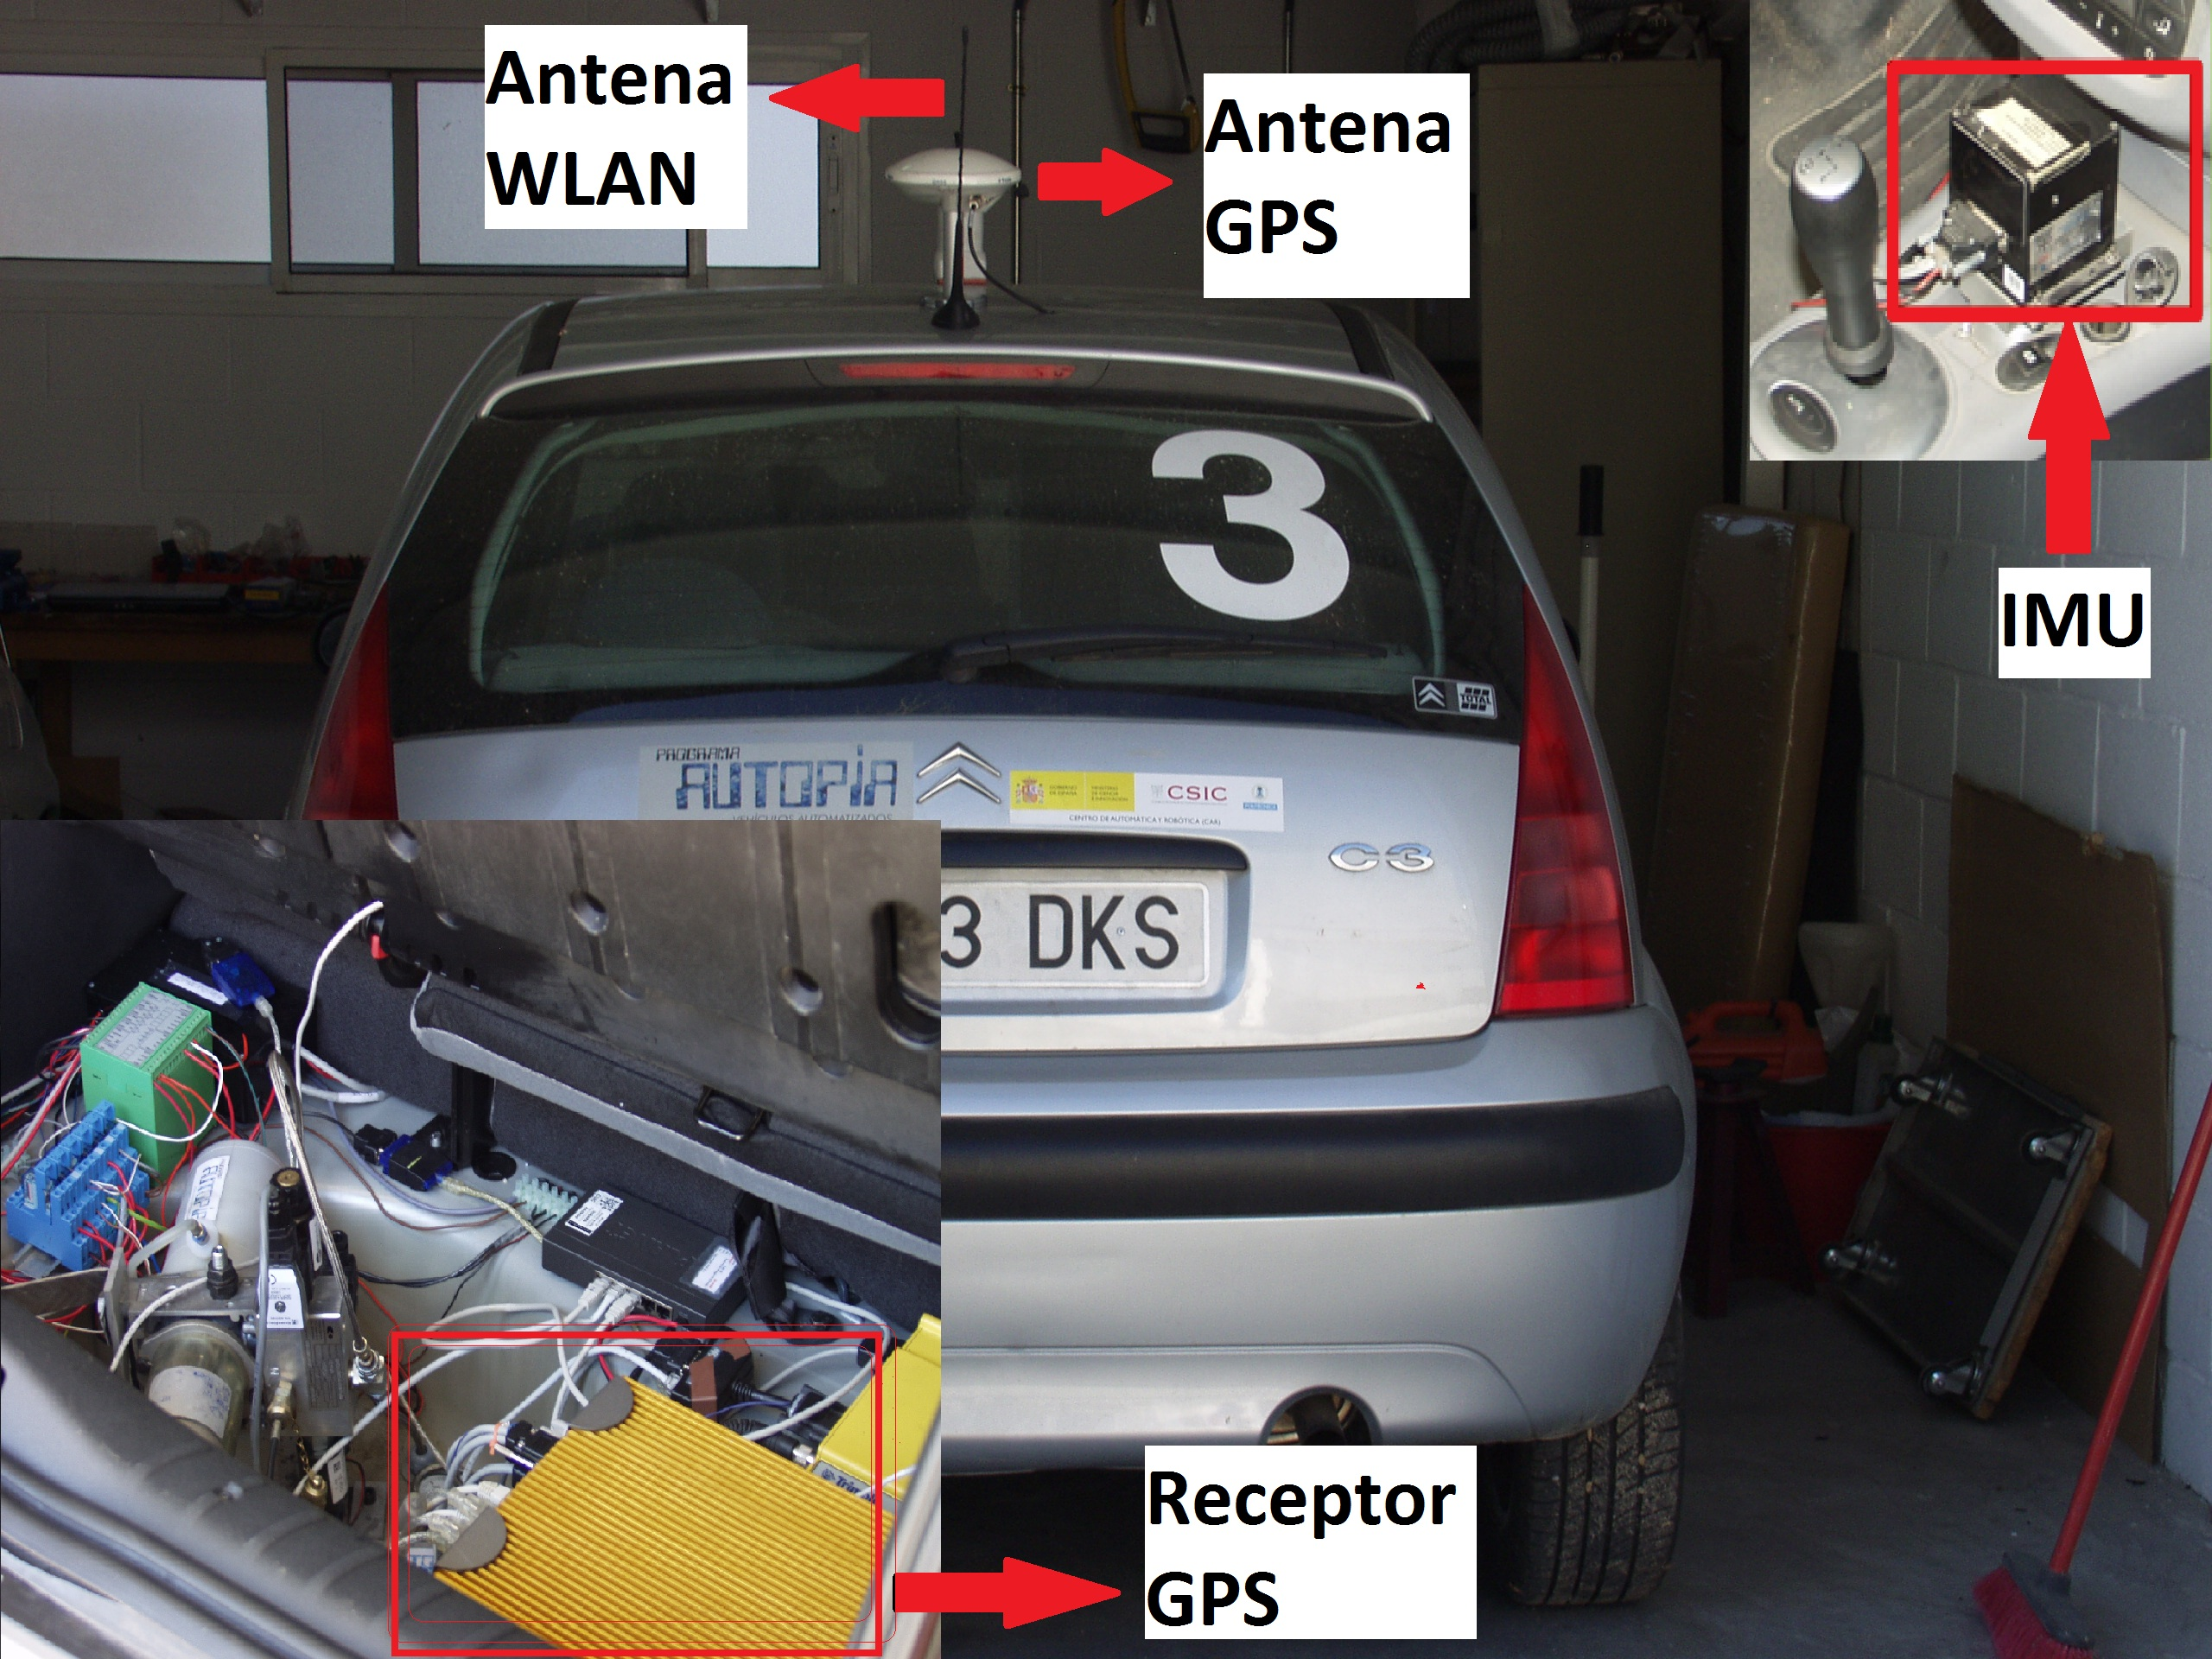
\includegraphics[width=0.9\linewidth]{figures/maletero.jpg}
\caption{Instrumentación de Platero}
\label{fig:maleta}
\end{minipage}
\end{figure} 
\interfootnotelinepenalty=10000
Platero está instrumentado para actuar sobre los pedales acelerador/freno y sobre volante, ambos sistemas pueden funcionar conjunta o independientemente. Posee un sistema de navegación, formado principalmente por un \gls{GPS}, un sistema para comunicarse con la estación base vía \gls{WLAN}, y un bus \gls{CAN}\footnote{Red interna del vehículo donde circulan mensajes y órdenes, tales como subir bajar ventanas, cambiar a segunda velocidad, encender luces intermitentes, ...}, del cual se obtienen variables, tales como la velocidad, aceleración,.. o bien se pueden recibir órdenes de control. En esta sección se enfoca en los controles de aceleración y freno, para un descripción más detallada de los otros sistemas de Platero, referirse a la sección \ref{ape:platero} del apéndice.

En lo que se refiere a la actuación necesaria para llevar a cabo un control de velocidad, se debe tener en cuenta únicamente el manejo de los pedales de acelerador y freno, dado que el vehículo utilizado (\textit{Platero}) dispone de su propio sistema de cambio de velocidades de la transmisión automático implementado por Citroën.

Para lograr el control sobre el \textbf{acelerador}, se cortaron las dos señales de tensión que genera el acelerador y se conmutaron por otras generadas por el ordenador embarcado del vehículo. Para el control del \textbf{freno}, se intervino la caja del \gls{ABS} con un sistema de actuación que consta de una válvula con una salida, conectada directamente al \gls{ABS} para respetar el circuito original. El sistema consta de dos entradas: la primera conectada al circuito inicial de freno, que permite su accionamiento convencional, y la segundo conectada a un sistema electro-hidráulico diseñado para el accionamiento automático del freno desde el ordenador embarcado.

Por otra parte, el funcionamiento de los sistemas de actuación no impide que un usuario pueda actuar sobre los pedales en caso de emergencia, o desactivarlos para realizar una conducción manual cuando lo desee. Con el sistema automático activado, el ordenador generará ordenes de control en el intervalo [0,1] que se traducirán en porcentaje de presión a aplicar sobre el correspondiente pedal.

\section{TORCS}
\label{sec:torcs}

\gls{TORCS} es un simulador de carros multiplataforma y altamente portable. Es utilizado como un juego ordinario de carreras, como un juego de carreras de inteligencia artificial y como una plataforma de investigación. Es compatible con \gls{Linux} (\gls{x86}, \gls{AMD64} y \gls{PPC}), \gls{FreeBSD}, \gls{MacOSX} y \gls{Windows}. El código fuente de TORCS esta licenciado bajo \gls{GPL}.

\begin{figure}[ht]
\begin{minipage}[b]{0.5\linewidth}
\centering
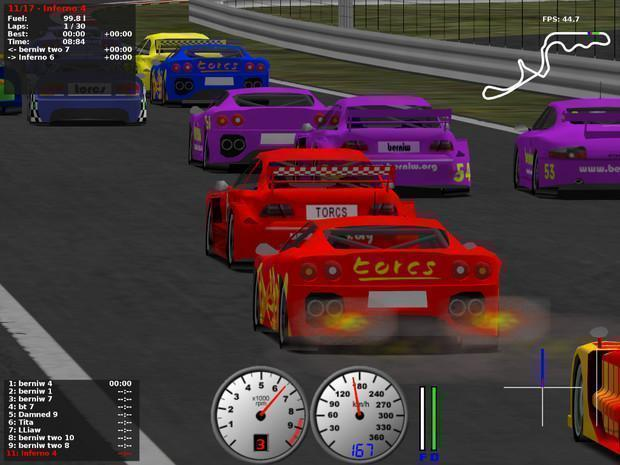
\includegraphics[width=0.7\linewidth]{figures/torcs_screenshot3.jpg}
\end{minipage}
\begin{minipage}[b]{0.5\linewidth}
\centering
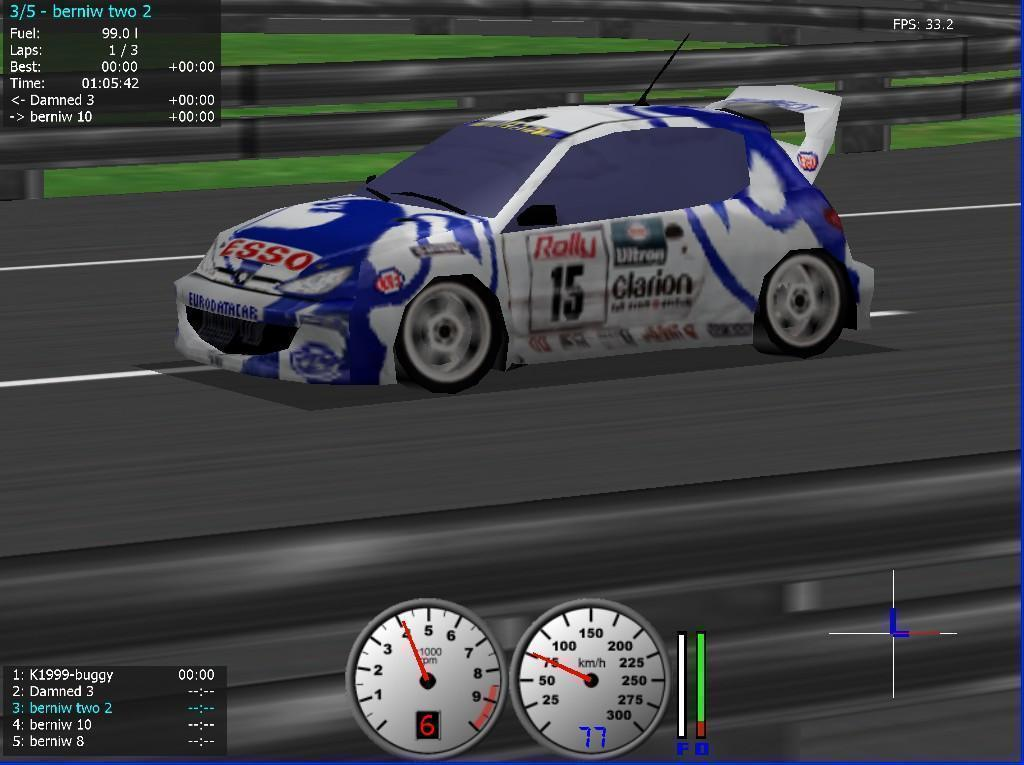
\includegraphics[width=0.7\linewidth]{figures/torcs3.jpg}
\end{minipage}
\caption{Captura de pantalla de \gls{TORCS}.}
\end{figure} 

A nivel de simulación posee un modelo de daños simple, colisiones, propiedades de frenado y ruedas (rigidez, humedad, brincos,…), aerodinámica (efecto del suelo, spoilers,…) y muchos más.

Lo elegimos como plataforma para realizar las simulaciones por varias razones: todo su código es \gls{Open Source}; la implementación del juego esta diseñada para facilitar al programador el desarrollo de robots inteligentes de una manera fácil y sencilla; un entorno gráfico agradable, sobre el cual se puede ver el comportamiento del vehículo; un modo texto, el cual reduce el tiempo de ejecución de las simulaciones considerablemente; un entorno virtual muy fiel a la realidad cumpliendo con la mayoría de las leyes físicas fundamentales como gravedad, coeficiente de fricción, aerodinámica, daños en el carro, consumo de combustible, balance de masa, etc.; más de 30 pistas distintas, de características muy dispares, anchura de pista, longitud, tipo de superficie, etc.; posibilidad de elegir entre casi 50 vehículos distintos.         
